Phages, small viruses that infect, replicate, and kill bacteria, are nature's natural anti-microbial defense. Research is currently being done to determine the applications of phages in controlling bacterial infections and spread. Phages have applications in human and animal health. Phage cocktails are a type of medicine for sick patients with bacterial diseases, such as \textit{E. coli}. A patient can intake a pill filled with specific phages that target \textit{E. coli}. The phages will target the specific \textit{E. coli} bacteria, but will not affect the other bacteria and will not have any side effects on the body. There are 100 trillion microbes across 5,000 different types of bacteria strains in the human gut. Using medicine such as antibiotics can disrupt the intricate ecosystem of the gut microbiome, acting as a scorched-earth mechanism. Phages on the other hand specifically target a specific bacterial strain, acting as a sniper, with minimal to no effects to other bacteria. This can be used to control bacterial infections and cure people, or to prevent the spread of common bacteria in livestock, which are commonly raised in tight spaces with a lack of sanitation facilities to clean out the feces and other junk of the livestock. 

Phages have applications in the food production business. Once an animal is slaughtered, bacteria start to grow and eventually spoil the meat. A possible way to prolong the shelf-life of meat is to use a solution of water with a mixture of phages and douse the meat with the solution. As the bacteria start to replicate, the phages kill the bacteria, slowing the growth down. An issue with this is that there are many types of bacteria, while phages can only target a select few bacteria strains. 

In an ecosystem like the ocean, the gut, or in soil, there are thousands of different microbes. The ecosystem is complex, with many different factors affecting the growth of bacteria, fungi,  phages, and more. External factors, such as flooding, droughts, or chemical spills have a massive impact on the ecosystem, adding or removing nutrients from the system, a change in temperature and pH of the ecosystem, or directly destroying microbes. These effects can affect the balance of microbes, affecting the larger ecosystem and food chain as a whole. For example, bacteria are used to decompose dead organic material into nutrients for the grass to grow, which is then eaten by rabbits who are eaten by eagles. 

Not much is known about phages in large and complex communities between other phages, bacteria, resources, and the environment. There have been previous attempts to model the complex dynamics of the populations between phages, bacteria, and resources, with the environment using Ordinary Differential Equations(ODE) and Delay Differential Equations (DDE). However, these methods have mainly stayed with 1-to-1-to-1 models, meaning 1 phage, 1 bacteria, and 1 resource. Other methods such as Partial Differential Equations (PDE) or cellular models have been created in an attempt to model these types of dynamics. There are two main ways to model phage-bacteria dynamics: a spatial model or a non-spatial one. A spatial model means that phages and bacteria can travel through space, while with non-spatial models the bacteria and phages are assumed to be in a well-mixed solution. Special considerations have to be accounted for with spatial models. Bacteria and phages can only interact in the proximity of one another, while in non-spatial models it is assumed that a set percentage $p$ interact with one another. Spatial models can potentially lead to more interesting and complex results but are limited to smaller populations and harder to develop, while non-spatial models are easier to develop and are more effective in modeling large populations. PDE and cellular models are types of spatial models, while ODEs and DDEs are types of non-spatial models \newline 

\subsection{Biological Background}
Phages are small viruses on the order of 27-190nm that infect and lysis (kill) specific bacteria. The phage cycle process starts by a phage coming into contact with a bacterium. Once it has identified an injection site, the phage can inject a strain of DNA into the bacteria. The DNA strand has two options, either it can merge into the DNA of the bacteria, so that when the bacteria replicates, the phage's DNA strand is replicated along with the bacteria. This stage is called the Lysogenic Cycle. After a set amount of time, the DNA of the phage can unmerge and hijack the DNA replicating mechanism, creating multiple copies of itself, using the transcription, translation, and replication process to create multiple copies of itself. The phages begin to self-assemble inside the bacteria until the bacteria is full of phages and explodes, the lysing stage, releasing the phages into the environment, ready to repeat the process again. 

This process can be visualized in \Cref{fig:phage_life_cycle}. \cite{campbellFutureBacteriophageBiology2003}
\begin{figure}
    \centering
    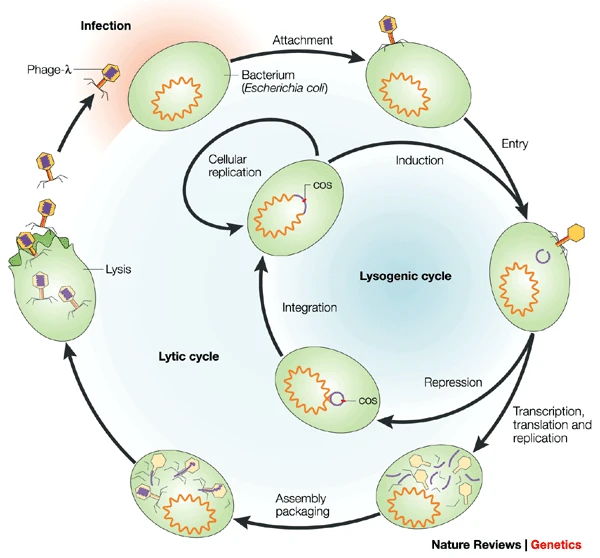
\includegraphics[width=0.5\linewidth]{Figures/phage_life_cycle.png}
    \caption{Life cycle of a phage inside and outside a bacteria cell.}
    \label{fig:phage_life_cycle}
\end{figure}

\subsection{Real World Applications of Phages}
Due to the nature of killing bacteria, there are numerous applications where a researcher or an organization might be interested in controlling bacterial populations. A Food Safety Specialist might be interested in introducing a solution containing a high concentration of phages during food production to prevent the spread and growth of \textit{Salmonella} or \textit{E. coli}, without affecting the quality of the food that other bacterial control methods like heat or acidity provide. The Food Safety Specialist might want to promote beneficial bacteria like \textit{Streptococcus thermophilus} used in the production of Emmantal cheese, which heat would also kill. A doctor might be interested in providing swallowable pills, more commonly known as phage cocktails, to a patient with a bacterial infection. The medication can contain any number of different phages that can target specific bacterial infections such as \textit{Streptococcus pneumoniae} with minimal risk of side effects. An Environmental Protection Officer might be interested to see how they can use phages to stop the spread of \textit{Cyanobacteria} blooms in waterways, more commonly known as blue-green algae, a photosynthetic microscopic organism that is technically a type of bacteria. This would keep waterways safe for boating and swimming activity, aquatic life, and water consumption in farms, factories, and homes. 


\subsubsection{Controlling Foodborne Bacteria}
Foodborne diseases are one of a few primary ways for bacteria to spread to humans and animals. Some bacteria directly infect the host, while some bacteria will deposit toxins on the food. If consumed in large enough quantities, the toxins can be fatal. Methods exist to control bacterial growth, for example by storing food below 5C or above 60C. Bacteria need moisture to grow, so starches like rice will have minimal bacterial growth. Bacteria prefer to live in slightly acidic to neutral pH environments, so having an environment that is extremely acidic like vinegar will prevent bacterial growth. The use of chemical antibacterial agents such as bleach are not desirable due to leaving chemicals on the food, which can be fatal if ingested. Physical agents like heat or radiation can kill bacteria, but at the cost of altering the food quality \cite{fieseler_food_2021}. 

\subsubsection{As an Alternative to Antibiotics}


\subsubsection{Environmental Protection}
Algae blooms, also called red tides, is the rapid spread of bacterial or algae organisms. Blooms are a growing environmental concern impacting water quality, aquatic ecosystems, and human health. These rapid increases in algae populations, often fueled by excess nutrients like nitrogen and phosphorus, can occur in freshwater, coastal, and marine environments. Algae blooms can produce toxins that threaten wildlife, contaminate drinking water, and disrupt local economies dependent on fishing and tourism. In the state of Florida, between the years 1995 and 2000, an estimated $\$6.5$ million was lost in the restaurant and hotel industry due to algae blooms. This accounts for about 25\% of the average total monthly sales revenue in the region from June through October, the months that are most commonly affected by red tide\cite{PDFEconomicImpacts}. During a red bloom event, hospital diagnoses in the county of Sarasota for pneumonia, gastrointestinal, and respiratory illness increased by 19\%, 40\% and 54\% respectively \cite{chengCharacterizationMarineAerosol2005, kirkpatrickGastrointestinalEmergencyRoom2010}, with a respiratory illness visit costing between $\$0.5\%$ and $\$4$ million \cite{hoaglandCostsRespiratoryIllnesses2009}. 

Cyanobacteria blooms have major effects on the aquatic environment as well as human health. Cyanobacteria release nitrogen and phosphorous, which the bacteria use to grow with oxygen, outpacing other aquatic growth, and killing aquatic marine life. Toxins can make their way into the food and water consumed by humans, causing muscle fatigue, respiratory issues, liver damage, and gastrointestinal issues \cite{zhangImpactCyanobacteriaBlooms2022}. \Cref{fig:cyanobacteria_bloom_cycle} shows the process of how cyanobacteria degrade and are absorbed into the environment, eventually making their way into the human body via various contact points. 
\begin{figure}
    \centering
    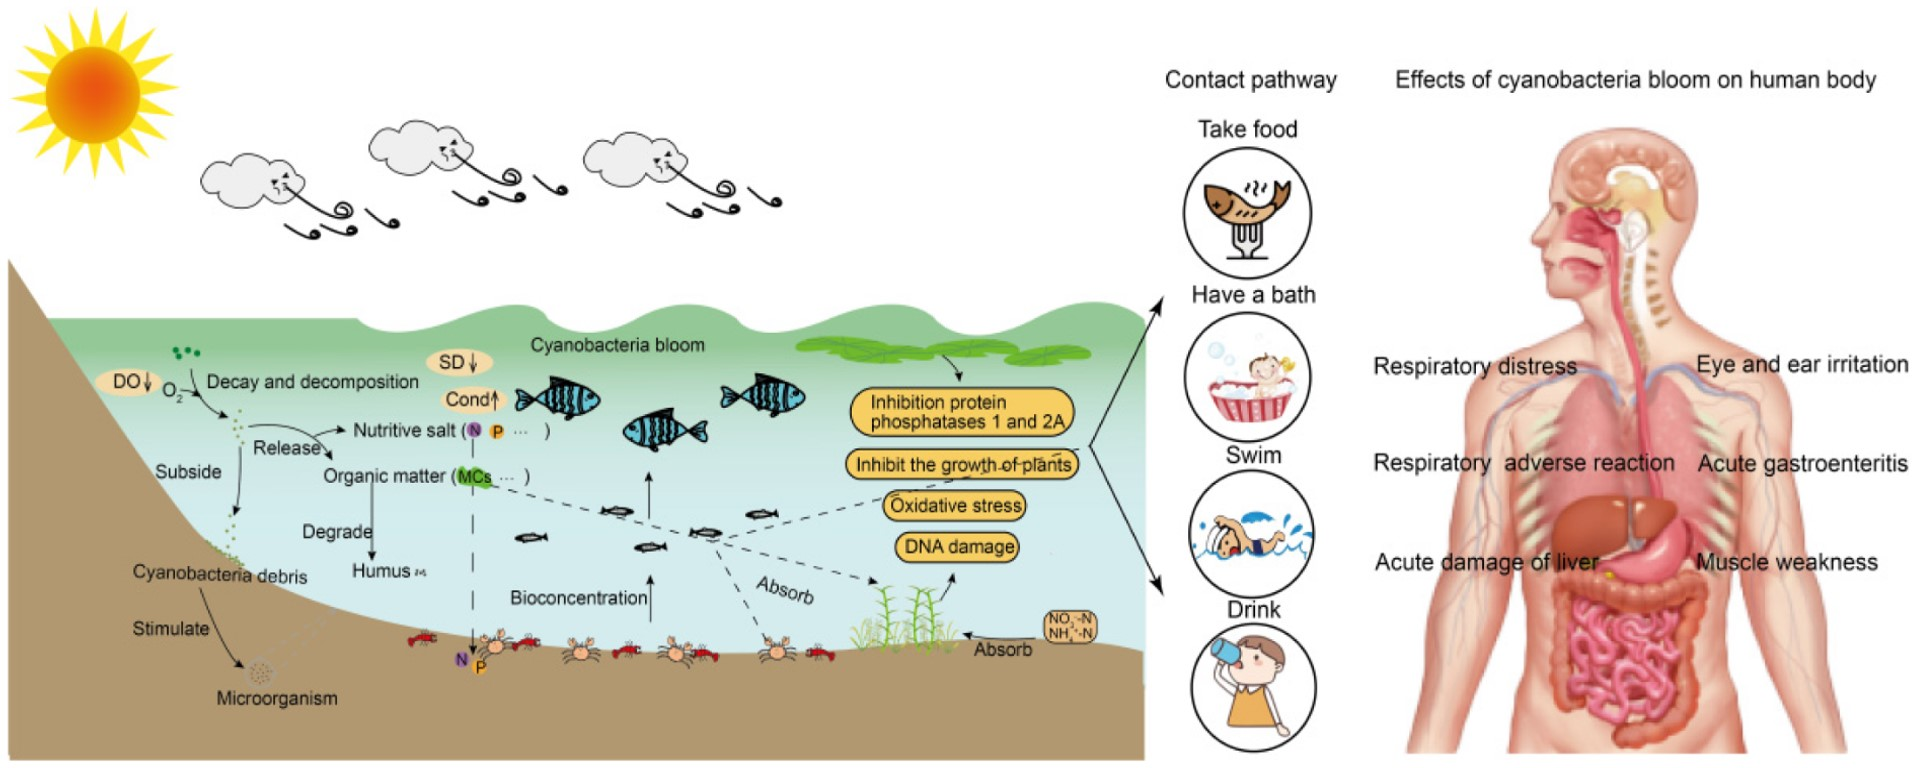
\includegraphics[width=0.75\linewidth]{Figures/cyanobacteria_bloom_cycle.png}
    \caption{Cyanobacteria degradation cycle, main hazards of cyanobacteria bloom to water bodies, aquatic organisms, and the human body. (DO: dissolved oxygen; SD: water transparency; Cond: conductivity; N: nitrogen; P: phosphorus; MCs: microcystins). \cite{zhangImpactCyanobacteriaBlooms2022}}
    \label{fig:cyanobacteria_bloom_cycle}
\end{figure}
